% Options for packages loaded elsewhere
\PassOptionsToPackage{unicode}{hyperref}
\PassOptionsToPackage{hyphens}{url}
%
\documentclass[
]{article}
\usepackage{amsmath,amssymb}
\usepackage{lmodern}
\usepackage{iftex}
\ifPDFTeX
  \usepackage[T1]{fontenc}
  \usepackage[utf8]{inputenc}
  \usepackage{textcomp} % provide euro and other symbols
\else % if luatex or xetex
  \usepackage{unicode-math}
  \defaultfontfeatures{Scale=MatchLowercase}
  \defaultfontfeatures[\rmfamily]{Ligatures=TeX,Scale=1}
\fi
% Use upquote if available, for straight quotes in verbatim environments
\IfFileExists{upquote.sty}{\usepackage{upquote}}{}
\IfFileExists{microtype.sty}{% use microtype if available
  \usepackage[]{microtype}
  \UseMicrotypeSet[protrusion]{basicmath} % disable protrusion for tt fonts
}{}
\makeatletter
\@ifundefined{KOMAClassName}{% if non-KOMA class
  \IfFileExists{parskip.sty}{%
    \usepackage{parskip}
  }{% else
    \setlength{\parindent}{0pt}
    \setlength{\parskip}{6pt plus 2pt minus 1pt}}
}{% if KOMA class
  \KOMAoptions{parskip=half}}
\makeatother
\usepackage{xcolor}
\usepackage[margin=1in]{geometry}
\usepackage{color}
\usepackage{fancyvrb}
\newcommand{\VerbBar}{|}
\newcommand{\VERB}{\Verb[commandchars=\\\{\}]}
\DefineVerbatimEnvironment{Highlighting}{Verbatim}{commandchars=\\\{\}}
% Add ',fontsize=\small' for more characters per line
\usepackage{framed}
\definecolor{shadecolor}{RGB}{248,248,248}
\newenvironment{Shaded}{\begin{snugshade}}{\end{snugshade}}
\newcommand{\AlertTok}[1]{\textcolor[rgb]{0.94,0.16,0.16}{#1}}
\newcommand{\AnnotationTok}[1]{\textcolor[rgb]{0.56,0.35,0.01}{\textbf{\textit{#1}}}}
\newcommand{\AttributeTok}[1]{\textcolor[rgb]{0.77,0.63,0.00}{#1}}
\newcommand{\BaseNTok}[1]{\textcolor[rgb]{0.00,0.00,0.81}{#1}}
\newcommand{\BuiltInTok}[1]{#1}
\newcommand{\CharTok}[1]{\textcolor[rgb]{0.31,0.60,0.02}{#1}}
\newcommand{\CommentTok}[1]{\textcolor[rgb]{0.56,0.35,0.01}{\textit{#1}}}
\newcommand{\CommentVarTok}[1]{\textcolor[rgb]{0.56,0.35,0.01}{\textbf{\textit{#1}}}}
\newcommand{\ConstantTok}[1]{\textcolor[rgb]{0.00,0.00,0.00}{#1}}
\newcommand{\ControlFlowTok}[1]{\textcolor[rgb]{0.13,0.29,0.53}{\textbf{#1}}}
\newcommand{\DataTypeTok}[1]{\textcolor[rgb]{0.13,0.29,0.53}{#1}}
\newcommand{\DecValTok}[1]{\textcolor[rgb]{0.00,0.00,0.81}{#1}}
\newcommand{\DocumentationTok}[1]{\textcolor[rgb]{0.56,0.35,0.01}{\textbf{\textit{#1}}}}
\newcommand{\ErrorTok}[1]{\textcolor[rgb]{0.64,0.00,0.00}{\textbf{#1}}}
\newcommand{\ExtensionTok}[1]{#1}
\newcommand{\FloatTok}[1]{\textcolor[rgb]{0.00,0.00,0.81}{#1}}
\newcommand{\FunctionTok}[1]{\textcolor[rgb]{0.00,0.00,0.00}{#1}}
\newcommand{\ImportTok}[1]{#1}
\newcommand{\InformationTok}[1]{\textcolor[rgb]{0.56,0.35,0.01}{\textbf{\textit{#1}}}}
\newcommand{\KeywordTok}[1]{\textcolor[rgb]{0.13,0.29,0.53}{\textbf{#1}}}
\newcommand{\NormalTok}[1]{#1}
\newcommand{\OperatorTok}[1]{\textcolor[rgb]{0.81,0.36,0.00}{\textbf{#1}}}
\newcommand{\OtherTok}[1]{\textcolor[rgb]{0.56,0.35,0.01}{#1}}
\newcommand{\PreprocessorTok}[1]{\textcolor[rgb]{0.56,0.35,0.01}{\textit{#1}}}
\newcommand{\RegionMarkerTok}[1]{#1}
\newcommand{\SpecialCharTok}[1]{\textcolor[rgb]{0.00,0.00,0.00}{#1}}
\newcommand{\SpecialStringTok}[1]{\textcolor[rgb]{0.31,0.60,0.02}{#1}}
\newcommand{\StringTok}[1]{\textcolor[rgb]{0.31,0.60,0.02}{#1}}
\newcommand{\VariableTok}[1]{\textcolor[rgb]{0.00,0.00,0.00}{#1}}
\newcommand{\VerbatimStringTok}[1]{\textcolor[rgb]{0.31,0.60,0.02}{#1}}
\newcommand{\WarningTok}[1]{\textcolor[rgb]{0.56,0.35,0.01}{\textbf{\textit{#1}}}}
\usepackage{graphicx}
\makeatletter
\def\maxwidth{\ifdim\Gin@nat@width>\linewidth\linewidth\else\Gin@nat@width\fi}
\def\maxheight{\ifdim\Gin@nat@height>\textheight\textheight\else\Gin@nat@height\fi}
\makeatother
% Scale images if necessary, so that they will not overflow the page
% margins by default, and it is still possible to overwrite the defaults
% using explicit options in \includegraphics[width, height, ...]{}
\setkeys{Gin}{width=\maxwidth,height=\maxheight,keepaspectratio}
% Set default figure placement to htbp
\makeatletter
\def\fps@figure{htbp}
\makeatother
\setlength{\emergencystretch}{3em} % prevent overfull lines
\providecommand{\tightlist}{%
  \setlength{\itemsep}{0pt}\setlength{\parskip}{0pt}}
\setcounter{secnumdepth}{-\maxdimen} % remove section numbering
\ifLuaTeX
  \usepackage{selnolig}  % disable illegal ligatures
\fi
\IfFileExists{bookmark.sty}{\usepackage{bookmark}}{\usepackage{hyperref}}
\IfFileExists{xurl.sty}{\usepackage{xurl}}{} % add URL line breaks if available
\urlstyle{same} % disable monospaced font for URLs
\hypersetup{
  pdftitle={FINAL PREDICTION},
  pdfauthor={Yuang Guo},
  hidelinks,
  pdfcreator={LaTeX via pandoc}}

\title{FINAL PREDICTION}
\author{Yuang Guo}
\date{2023-11-01}

\begin{document}
\maketitle

\#ENV PREP

\begin{Shaded}
\begin{Highlighting}[]
  \FunctionTok{rm}\NormalTok{(}\AttributeTok{list =} \FunctionTok{ls}\NormalTok{()) }\CommentTok{\# Clear all files from your environment}
  \FunctionTok{gc}\NormalTok{()            }\CommentTok{\# Clear unused memory}
\end{Highlighting}
\end{Shaded}

\begin{verbatim}
##          used (Mb) gc trigger (Mb) max used (Mb)
## Ncells 475088 25.4    1027201 54.9   660385 35.3
## Vcells 882927  6.8    8388608 64.0  1771562 13.6
\end{verbatim}

\begin{Shaded}
\begin{Highlighting}[]
  \FunctionTok{cat}\NormalTok{(}\StringTok{"}\SpecialCharTok{\textbackslash{}f}\StringTok{"}\NormalTok{)       }\CommentTok{\# Clear the console}
\end{Highlighting}
\end{Shaded}

\newpage{}

\begin{Shaded}
\begin{Highlighting}[]
  \FunctionTok{graphics.off}\NormalTok{()  }\CommentTok{\# Clear all graphs}
\end{Highlighting}
\end{Shaded}

\begin{Shaded}
\begin{Highlighting}[]
\NormalTok{packages }\OtherTok{\textless{}{-}} \FunctionTok{c}\NormalTok{(}\StringTok{"psych"}\NormalTok{,       }\CommentTok{\# quick summary stats for data exploration,}
              \StringTok{"stargazer"}\NormalTok{,   }\CommentTok{\# summary stats,}
              \StringTok{"summarytools"}\NormalTok{,}\CommentTok{\# summary stats,}
              \StringTok{"naniar"}\NormalTok{,      }\CommentTok{\# for visualisation of missing data,}
              \StringTok{"visdat"}\NormalTok{,      }\CommentTok{\# for visualisation of missing data,}
              \StringTok{"VIM"}\NormalTok{,         }\CommentTok{\# for visualisation of missing data,}
              \StringTok{"DataExplorer"}\NormalTok{,}\CommentTok{\# for visualisation of missing data,}
              \StringTok{"tidyverse"}\NormalTok{,   }\CommentTok{\# data manipulation like selecting variables,}
              \StringTok{"fastDummies"}\NormalTok{, }\CommentTok{\# Create dummy variables using fastDummies,}
              \StringTok{"corrplot"}\NormalTok{,    }\CommentTok{\# correlation plots,}
              \StringTok{"ggplot2"}\NormalTok{,     }\CommentTok{\# graphing,}
              \StringTok{"data.table"}\NormalTok{,  }\CommentTok{\# reshape for graphing, }
              \StringTok{"car"}\NormalTok{,}
              \StringTok{"seasonal"}\NormalTok{,}
              \StringTok{"fpp3"}\NormalTok{,}
              \StringTok{"tsibble"}\NormalTok{,    }\CommentTok{\# vif for multicollinearity}
              \StringTok{"cli"}\NormalTok{,}
              \StringTok{"crayon"}\NormalTok{,}
              \StringTok{"dplyr"}\NormalTok{,}
              \StringTok{"fable"}\NormalTok{,}
              \StringTok{"fabletools"}\NormalTok{,}
              \StringTok{"feasts"}\NormalTok{,}
              \StringTok{"lubridate"}\NormalTok{,}
              \StringTok{"magrittr"}\NormalTok{,}
              \StringTok{"purrr"}\NormalTok{,}
              \StringTok{"rstudioapi"}\NormalTok{,}
              \StringTok{"tibble"}\NormalTok{,}
              \StringTok{"tidyr"}\NormalTok{,}
              \StringTok{"tsibbledata"}\NormalTok{,}
              \StringTok{"latex2exp"}\NormalTok{,}
              \StringTok{"GGally"}\NormalTok{,}
              \StringTok{"broom"}\NormalTok{,}
              \StringTok{"zoo"}\NormalTok{,}
              \StringTok{"caret"}\NormalTok{,}
              \StringTok{"xts"}
\NormalTok{              )}


\ControlFlowTok{for}\NormalTok{ (i }\ControlFlowTok{in} \DecValTok{1}\SpecialCharTok{:}\FunctionTok{length}\NormalTok{(packages)) \{}
  \ControlFlowTok{if}\NormalTok{ (}\SpecialCharTok{!}\NormalTok{packages[i] }\SpecialCharTok{\%in\%} \FunctionTok{rownames}\NormalTok{(}\FunctionTok{installed.packages}\NormalTok{())) \{}
    \FunctionTok{install.packages}\NormalTok{(packages[i]}
\NormalTok{                     , }\AttributeTok{repos =} \StringTok{"http://cran.rstudio.com/"}
\NormalTok{                     , }\AttributeTok{dependencies =} \ConstantTok{TRUE}
\NormalTok{                     )}
\NormalTok{  \}}
  \FunctionTok{library}\NormalTok{(packages[i], }\AttributeTok{character.only =} \ConstantTok{TRUE}\NormalTok{)}
\NormalTok{\}}
\end{Highlighting}
\end{Shaded}

\begin{verbatim}
## 
## Please cite as:
\end{verbatim}

\begin{verbatim}
##  Hlavac, Marek (2022). stargazer: Well-Formatted Regression and Summary Statistics Tables.
\end{verbatim}

\begin{verbatim}
##  R package version 5.2.3. https://CRAN.R-project.org/package=stargazer
\end{verbatim}

\begin{verbatim}
## Loading required package: colorspace
\end{verbatim}

\begin{verbatim}
## Loading required package: grid
\end{verbatim}

\begin{verbatim}
## VIM is ready to use.
\end{verbatim}

\begin{verbatim}
## Suggestions and bug-reports can be submitted at: https://github.com/statistikat/VIM/issues
\end{verbatim}

\begin{verbatim}
## 
## Attaching package: 'VIM'
\end{verbatim}

\begin{verbatim}
## The following object is masked from 'package:datasets':
## 
##     sleep
\end{verbatim}

\begin{verbatim}
## -- Attaching core tidyverse packages ------------------------ tidyverse 2.0.0 --
## v dplyr     1.1.3     v readr     2.1.4
## v forcats   1.0.0     v stringr   1.5.0
## v ggplot2   3.4.4     v tibble    3.2.1
## v lubridate 1.9.3     v tidyr     1.3.0
## v purrr     1.0.2     
## -- Conflicts ------------------------------------------ tidyverse_conflicts() --
## x ggplot2::%+%()   masks psych::%+%()
## x ggplot2::alpha() masks psych::alpha()
## x dplyr::filter()  masks stats::filter()
## x dplyr::lag()     masks stats::lag()
## x tibble::view()   masks summarytools::view()
## i Use the conflicted package (<http://conflicted.r-lib.org/>) to force all conflicts to become errors
## Thank you for using fastDummies!
## 
## To acknowledge our work, please cite the package:
## 
## Kaplan, J. & Schlegel, B. (2023). fastDummies: Fast Creation of Dummy (Binary) Columns and Rows from Categorical Variables. Version 1.7.1. URL: https://github.com/jacobkap/fastDummies, https://jacobkap.github.io/fastDummies/.
## 
## corrplot 0.92 loaded
## 
## 
## Attaching package: 'data.table'
## 
## 
## The following objects are masked from 'package:lubridate':
## 
##     hour, isoweek, mday, minute, month, quarter, second, wday, week,
##     yday, year
## 
## 
## The following objects are masked from 'package:dplyr':
## 
##     between, first, last
## 
## 
## The following object is masked from 'package:purrr':
## 
##     transpose
## 
## 
## Loading required package: carData
## 
## 
## Attaching package: 'car'
## 
## 
## The following object is masked from 'package:dplyr':
## 
##     recode
## 
## 
## The following object is masked from 'package:purrr':
## 
##     some
## 
## 
## The following object is masked from 'package:psych':
## 
##     logit
## 
## 
## 
## Attaching package: 'seasonal'
## 
## 
## The following object is masked from 'package:tibble':
## 
##     view
## 
## 
## The following object is masked from 'package:summarytools':
## 
##     view
## 
## 
## The following object is masked from 'package:psych':
## 
##     outlier
## 
## 
## -- Attaching packages ---------------------------------------------- fpp3 0.5 --
## 
## v tsibble     1.1.3     v fable       0.3.3
## v tsibbledata 0.4.1     v fabletools  0.3.4
## v feasts      0.3.1     
## 
## -- Conflicts ------------------------------------------------- fpp3_conflicts --
## x ggplot2::%+%()          masks psych::%+%()
## x ggplot2::alpha()        masks psych::alpha()
## x data.table::between()   masks dplyr::between()
## x lubridate::date()       masks base::date()
## x dplyr::filter()         masks stats::filter()
## x data.table::first()     masks dplyr::first()
## x data.table::hour()      masks lubridate::hour()
## x tsibble::intersect()    masks base::intersect()
## x tsibble::interval()     masks lubridate::interval()
## x data.table::isoweek()   masks lubridate::isoweek()
## x tsibble::key()          masks data.table::key()
## x dplyr::lag()            masks stats::lag()
## x data.table::last()      masks dplyr::last()
## x data.table::mday()      masks lubridate::mday()
## x data.table::minute()    masks lubridate::minute()
## x data.table::month()     masks lubridate::month()
## x data.table::quarter()   masks lubridate::quarter()
## x car::recode()           masks dplyr::recode()
## x data.table::second()    masks lubridate::second()
## x tsibble::setdiff()      masks base::setdiff()
## x car::some()             masks purrr::some()
## x data.table::transpose() masks purrr::transpose()
## x tsibble::union()        masks base::union()
## x seasonal::view()        masks tibble::view(), summarytools::view()
## x data.table::wday()      masks lubridate::wday()
## x data.table::week()      masks lubridate::week()
## x data.table::yday()      masks lubridate::yday()
## x data.table::year()      masks lubridate::year()
## 
## 
## Attaching package: 'crayon'
## 
## 
## The following object is masked from 'package:cli':
## 
##     num_ansi_colors
## 
## 
## The following object is masked from 'package:ggplot2':
## 
##     %+%
## 
## 
## The following object is masked from 'package:psych':
## 
##     %+%
## 
## 
## 
## Attaching package: 'magrittr'
## 
## 
## The following object is masked from 'package:purrr':
## 
##     set_names
## 
## 
## The following object is masked from 'package:tidyr':
## 
##     extract
## 
## 
## Registered S3 method overwritten by 'GGally':
##   method from   
##   +.gg   ggplot2
## 
## 
## Attaching package: 'zoo'
## 
## 
## The following object is masked from 'package:tsibble':
## 
##     index
## 
## 
## The following objects are masked from 'package:base':
## 
##     as.Date, as.Date.numeric
## 
## 
## Loading required package: lattice
## 
## 
## Attaching package: 'caret'
## 
## 
## The following objects are masked from 'package:fabletools':
## 
##     MAE, RMSE
## 
## 
## The following object is masked from 'package:purrr':
## 
##     lift
## 
## 
## 
## ######################### Warning from 'xts' package ##########################
## #                                                                             #
## # The dplyr lag() function breaks how base R's lag() function is supposed to  #
## # work, which breaks lag(my_xts). Calls to lag(my_xts) that you type or       #
## # source() into this session won't work correctly.                            #
## #                                                                             #
## # Use stats::lag() to make sure you're not using dplyr::lag(), or you can add #
## # conflictRules('dplyr', exclude = 'lag') to your .Rprofile to stop           #
## # dplyr from breaking base R's lag() function.                                #
## #                                                                             #
## # Code in packages is not affected. It's protected by R's namespace mechanism #
## # Set `options(xts.warn_dplyr_breaks_lag = FALSE)` to suppress this warning.  #
## #                                                                             #
## ###############################################################################
## 
## 
## Attaching package: 'xts'
## 
## 
## The following objects are masked from 'package:data.table':
## 
##     first, last
## 
## 
## The following objects are masked from 'package:dplyr':
## 
##     first, last
\end{verbatim}

\begin{Shaded}
\begin{Highlighting}[]
\FunctionTok{rm}\NormalTok{(packages)}
\end{Highlighting}
\end{Shaded}

\#import data

\begin{Shaded}
\begin{Highlighting}[]
\FunctionTok{setwd}\NormalTok{(}\FunctionTok{getwd}\NormalTok{())}
\NormalTok{rawdata }\OtherTok{=} \FunctionTok{read.csv}\NormalTok{(}\StringTok{"petfood\_retail\_table.csv"}\NormalTok{)}
\end{Highlighting}
\end{Shaded}

\#create tsibble for FMCG

\begin{Shaded}
\begin{Highlighting}[]
\NormalTok{manu\_fmcg }\OtherTok{\textless{}{-}}\NormalTok{ rawdata }\SpecialCharTok{|\textgreater{}} \FunctionTok{filter}\NormalTok{(MANU\_ID }\SpecialCharTok{==} \StringTok{"MARS"}\NormalTok{) }\SpecialCharTok{|\textgreater{}} 
                        \FunctionTok{mutate}\NormalTok{(}\AttributeTok{DATE =} \FunctionTok{yearmonth}\NormalTok{(DATE)) }\SpecialCharTok{|\textgreater{}}
                        \FunctionTok{mutate}\NormalTok{(}\AttributeTok{transaction =}\NormalTok{ PRICE}\SpecialCharTok{*}\NormalTok{UNITS) }\SpecialCharTok{|\textgreater{}}  
                        \FunctionTok{group\_by}\NormalTok{(DATE) }\SpecialCharTok{|\textgreater{}}
                        \FunctionTok{summarise}\NormalTok{(}\AttributeTok{transaction =} \FunctionTok{sum}\NormalTok{(transaction))}

\NormalTok{manu\_fmcg\_monthly\_tsibble }\OtherTok{\textless{}{-}} \FunctionTok{as\_tsibble}\NormalTok{(manu\_fmcg, }\AttributeTok{index =} \StringTok{"DATE"}\NormalTok{)}
\NormalTok{manu\_fmcg\_monthly\_tsibble}
\end{Highlighting}
\end{Shaded}

\begin{verbatim}
## # A tsibble: 42 x 2 [1M]
##        DATE transaction
##       <mth>       <dbl>
##  1 2019 Jul       256. 
##  2 2019 Aug       188. 
##  3 2019 Sep       205. 
##  4 2019 Oct       148. 
##  5 2019 Nov        96.8
##  6 2019 Dec       198. 
##  7 2020 Jan       114. 
##  8 2020 Feb        78.9
##  9 2020 Mar       231. 
## 10 2020 Apr        82.9
## # i 32 more rows
\end{verbatim}

\#\#gg\_tsdisplay for original data

\begin{Shaded}
\begin{Highlighting}[]
\NormalTok{manu\_fmcg\_monthly\_tsibble }\SpecialCharTok{|\textgreater{}} \FunctionTok{filter}\NormalTok{(}\SpecialCharTok{!}\FunctionTok{is.na}\NormalTok{(transaction)) }\SpecialCharTok{|\textgreater{}}                                                                                \FunctionTok{gg\_tsdisplay}\NormalTok{(transaction,}\AttributeTok{plot\_type =} \StringTok{"partial"}\NormalTok{)}
\end{Highlighting}
\end{Shaded}

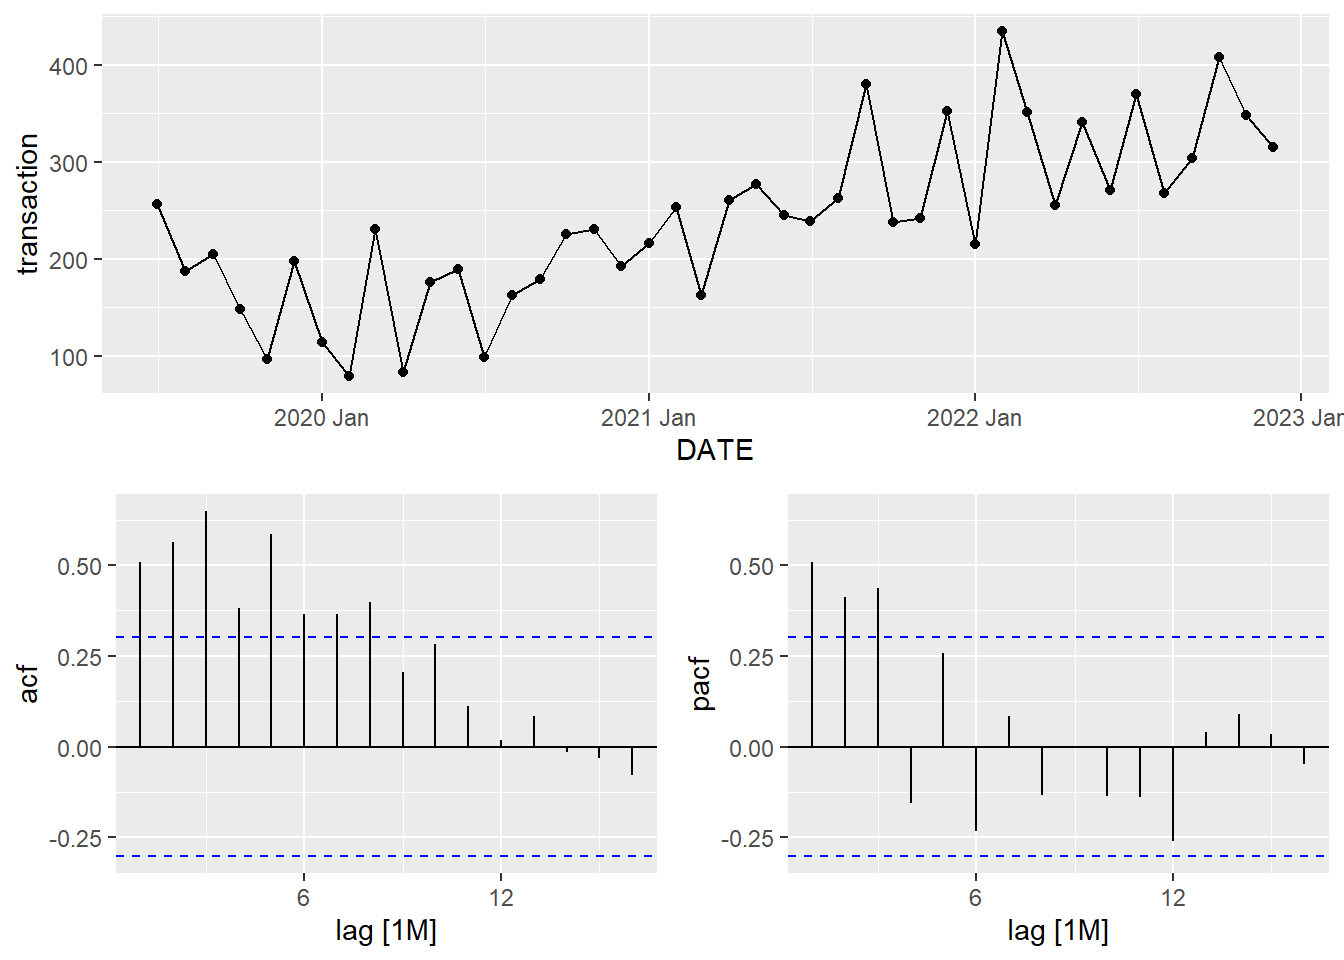
\includegraphics{FINAL_PREDICTION_files/figure-latex/unnamed-chunk-5-1.pdf}

\#\#decompostion for the original data

\begin{Shaded}
\begin{Highlighting}[]
\NormalTok{monthly\_dcmp }\OtherTok{\textless{}{-}}\NormalTok{ manu\_fmcg\_monthly\_tsibble }\SpecialCharTok{|\textgreater{}} \FunctionTok{filter}\NormalTok{(}\SpecialCharTok{!}\FunctionTok{is.na}\NormalTok{(transaction)) }\SpecialCharTok{|\textgreater{}}
                \FunctionTok{model}\NormalTok{(}\AttributeTok{stl =} \FunctionTok{STL}\NormalTok{(transaction))}
\FunctionTok{components}\NormalTok{(monthly\_dcmp) }\SpecialCharTok{|\textgreater{}} \FunctionTok{autoplot}\NormalTok{() }\SpecialCharTok{+} \FunctionTok{labs}\NormalTok{(}\AttributeTok{x =} \StringTok{"Year{-}Month"}\NormalTok{, }\AttributeTok{y =} \StringTok{"transaction"}\NormalTok{)}
\end{Highlighting}
\end{Shaded}

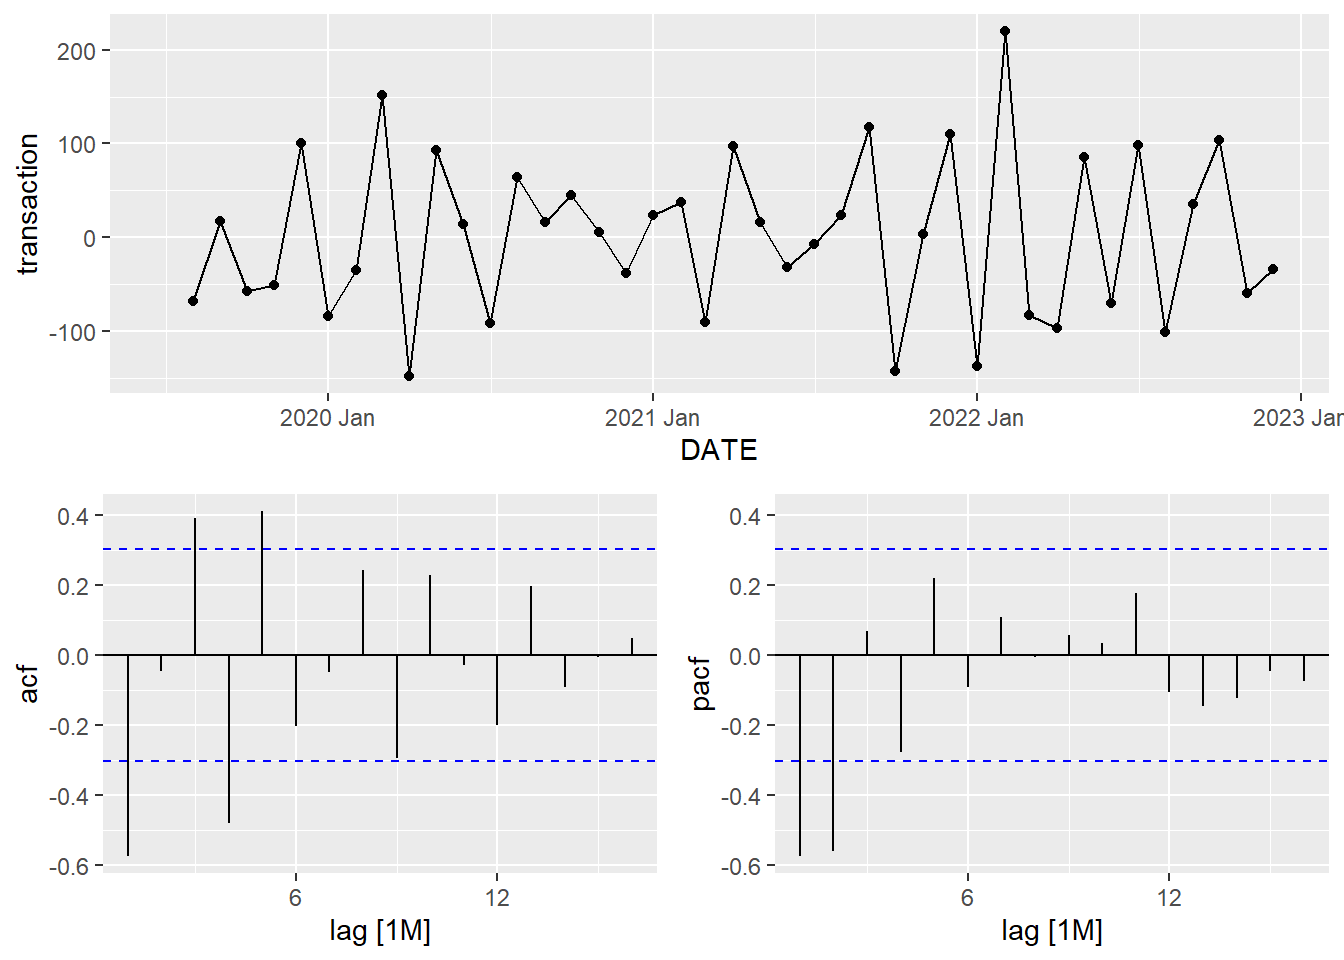
\includegraphics{FINAL_PREDICTION_files/figure-latex/unnamed-chunk-6-1.pdf}
\#\#check the seasonality

\begin{Shaded}
\begin{Highlighting}[]
\FunctionTok{Box.test}\NormalTok{(manu\_fmcg\_monthly\_tsibble}\SpecialCharTok{$}\NormalTok{transaction, }\AttributeTok{type =} \StringTok{"Ljung{-}Box"}\NormalTok{)}
\end{Highlighting}
\end{Shaded}

\begin{verbatim}
## 
##  Box-Ljung test
## 
## data:  manu_fmcg_monthly_tsibble$transaction
## X-squared = 11.672, df = 1, p-value = 0.0006345
\end{verbatim}

You should add seasonality in the prediction

\#\#autoarima model

\begin{Shaded}
\begin{Highlighting}[]
\NormalTok{model }\OtherTok{\textless{}{-}}\NormalTok{ forecast}\SpecialCharTok{::}\FunctionTok{auto.arima}\NormalTok{(manu\_fmcg\_monthly\_tsibble, }\AttributeTok{stepwise =} \ConstantTok{FALSE}\NormalTok{, }\AttributeTok{approximation =} \ConstantTok{FALSE}\NormalTok{, }\AttributeTok{seasonal =} \ConstantTok{TRUE}\NormalTok{)}
\end{Highlighting}
\end{Shaded}

\begin{verbatim}
## Registered S3 method overwritten by 'quantmod':
##   method            from
##   as.zoo.data.frame zoo
\end{verbatim}

\#\#summary of that model

\begin{Shaded}
\begin{Highlighting}[]
\FunctionTok{summary}\NormalTok{(model)}
\end{Highlighting}
\end{Shaded}

\begin{verbatim}
## Series: manu_fmcg_monthly_tsibble 
## ARIMA(2,1,0)(1,0,0)[12] 
## 
## Coefficients:
##           ar1      ar2     sar1
##       -0.9249  -0.5523  -0.3537
## s.e.   0.1255   0.1256   0.1717
## 
## sigma^2 = 3029:  log likelihood = -222.34
## AIC=452.67   AICc=453.78   BIC=459.53
## 
## Training set error measures:
##                    ME    RMSE      MAE       MPE     MAPE     MASE         ACF1
## Training set 8.373443 52.3515 40.08884 -2.267692 18.48982 0.442327 -0.003531046
\end{verbatim}

AR: yt - yt-1 = φ1(yt-1 - yt-2) + φ2(yt-2 - yt-3) + et et = yt - yt-1 -
φ1(yt-1 - yt-2) - φ2(yt-2 - yt-3)

SAR{[}12{]}: yt = et - Φ1B12yt yt = et - Φ1 yt-12\\
et = yt + Φ1 yt-12

Expaination of this model: (1 - φ1B - φ2B2)(1 - B)(1 - Φ1B12)yt = et
φ1:-0.9249 φ2:-0.5523 Φ1:-0.3537 This is our prediction function!
This type CANNOT be transformed to ETS

\#\#summary model for arima 210

\begin{Shaded}
\begin{Highlighting}[]
\CommentTok{\#model\_1 \textless{}{-} ARIMA(manu\_fmcg\_monthly\_tsibble, order = c(2,1,0))}
\NormalTok{model\_1 }\OtherTok{\textless{}{-}} \FunctionTok{arima}\NormalTok{(manu\_fmcg\_monthly\_tsibble}\SpecialCharTok{$}\NormalTok{transaction , }\AttributeTok{order =} \FunctionTok{c}\NormalTok{(}\DecValTok{2}\NormalTok{,}\DecValTok{1}\NormalTok{,}\DecValTok{0}\NormalTok{))}
\NormalTok{model\_1}
\end{Highlighting}
\end{Shaded}

\begin{verbatim}
## 
## Call:
## arima(x = manu_fmcg_monthly_tsibble$transaction, order = c(2, 1, 0))
## 
## Coefficients:
##           ar1      ar2
##       -0.9147  -0.5744
## s.e.   0.1269   0.1241
## 
## sigma^2 estimated as 3187:  log likelihood = -224.16,  aic = 454.31
\end{verbatim}

\#\#Confidence Interval for Forecast

\begin{Shaded}
\begin{Highlighting}[]
\NormalTok{forecast\_arima }\OtherTok{\textless{}{-}} \FunctionTok{forecast}\NormalTok{(forecast}\SpecialCharTok{::}\FunctionTok{auto.arima}\NormalTok{(manu\_fmcg\_monthly\_tsibble, }\AttributeTok{stepwise =} \ConstantTok{FALSE}\NormalTok{, }\AttributeTok{approximation =} \ConstantTok{FALSE}\NormalTok{, }\AttributeTok{seasonal =} \ConstantTok{TRUE}\NormalTok{), }\AttributeTok{h =} \DecValTok{24}\NormalTok{)}
\NormalTok{forecast\_arima}
\end{Highlighting}
\end{Shaded}

\begin{verbatim}
##          Point Forecast    Lo 80    Hi 80    Lo 95    Hi 95
## Jan 2023       390.2214 319.6875 460.7553 282.3491 498.0937
## Feb 2023       284.6388 213.9064 355.3713 176.4629 392.8148
## Mar 2023       325.0023 249.4063 400.5983 209.3883 440.6164
## Apr 2023       364.2830 277.3455 451.2205 231.3235 497.2425
## May 2023       322.9356 234.5220 411.3492 187.7186 458.1526
## Jun 2023       355.0248 261.0190 449.0305 211.2554 498.7942
## Jul 2023       319.5221 220.1846 418.8595 167.5986 471.4455
## Aug 2023       351.9698 249.9599 453.9797 195.9592 507.9804
## Sep 2023       342.8266 236.1096 449.5437 179.6170 506.0363
## Oct 2023       304.7467 194.2300 415.2634 135.7260 473.7674
## Nov 2023       325.0898 211.4058 438.7738 151.2251 498.9545
## Dec 2023       338.2101 220.6297 455.7905 158.3864 518.0338
## Jan 2024       310.6915 193.0701 428.3128 130.8052 490.5777
## Feb 2024       348.1087 227.6186 468.5988 163.8350 532.3824
## Mar 2024       334.2614 212.1717 456.3510 147.5413 520.9814
## Apr 2024       319.9305 197.1580 442.7030 132.1662 507.6948
## May 2024       334.7223 209.8606 459.5841 143.7628 525.6819
## Jun 2024       323.4591 197.3900 449.5282 130.6531 516.2652
## Jul 2024       335.8440 208.6441 463.0439 141.3086 530.3795
## Aug 2024       324.4787 195.6661 453.2913 127.4769 521.4806
## Sep 2024       327.7048 197.7163 457.6933 128.9046 526.5050
## Oct 2024       341.1196 209.8593 472.3798 140.3743 541.8648
## Nov 2024       333.9787 201.3374 466.6200 131.1213 536.8361
## Dec 2024       329.3175 195.4791 463.1558 124.6294 534.0056
\end{verbatim}

\#\#Create teh prediction graph

\begin{Shaded}
\begin{Highlighting}[]
\NormalTok{manu\_fmcg\_monthly\_tsibble }\SpecialCharTok{|\textgreater{}}
    \FunctionTok{model}\NormalTok{(}\AttributeTok{auto\_arima =} \FunctionTok{ARIMA}\NormalTok{(transaction }\SpecialCharTok{\textasciitilde{}} \FunctionTok{pdq}\NormalTok{(}\DecValTok{2}\NormalTok{,}\DecValTok{1}\NormalTok{,}\DecValTok{0}\NormalTok{) }\SpecialCharTok{+} \FunctionTok{PDQ}\NormalTok{(}\DecValTok{1}\NormalTok{,}\DecValTok{0}\NormalTok{,}\DecValTok{0}\NormalTok{,}\DecValTok{12}\NormalTok{))) }\SpecialCharTok{|\textgreater{}}
    \FunctionTok{forecast}\NormalTok{(}\AttributeTok{h =} \DecValTok{24}\NormalTok{) }\SpecialCharTok{|\textgreater{}}
    \FunctionTok{autoplot}\NormalTok{(manu\_fmcg\_monthly\_tsibble) }\SpecialCharTok{+}
    \FunctionTok{labs}\NormalTok{(}
         \AttributeTok{title =} \StringTok{"Prediction for FMCG in 2 years from 2023 JAN to 2024 DEC"}\NormalTok{,}
         \AttributeTok{x =} \StringTok{"Year{-}Month"}\NormalTok{,}
         \AttributeTok{y =} \StringTok{"total transaction per month ($)"}\NormalTok{,}
\NormalTok{         )}
\end{Highlighting}
\end{Shaded}

\includegraphics{FINAL_PREDICTION_files/figure-latex/unnamed-chunk-12-1.pdf}

\#\#metrics(using cv) from that we have 48 period of data, what if we
add cv in R, but I know it's very easy in python I think LOOCV is better
\#I will turn to python for the prediction

\#\#write the data out for python

\begin{Shaded}
\begin{Highlighting}[]
\CommentTok{\# Export data to a CSV file using write.table}
\NormalTok{file\_path }\OtherTok{\textless{}{-}} \StringTok{"C:}\SpecialCharTok{\textbackslash{}\textbackslash{}}\StringTok{Users}\SpecialCharTok{\textbackslash{}\textbackslash{}}\StringTok{guoyy}\SpecialCharTok{\textbackslash{}\textbackslash{}}\StringTok{OneDrive}\SpecialCharTok{\textbackslash{}\textbackslash{}}\StringTok{Desktop}\SpecialCharTok{\textbackslash{}\textbackslash{}}\StringTok{Program}\SpecialCharTok{\textbackslash{}\textbackslash{}}\StringTok{Mars\_petcare}\SpecialCharTok{\textbackslash{}\textbackslash{}}\StringTok{me}\SpecialCharTok{\textbackslash{}\textbackslash{}}\StringTok{ts\_cv.csv"}
\FunctionTok{write.table}\NormalTok{(manu\_fmcg\_monthly\_tsibble, }
            \AttributeTok{file =}\NormalTok{ file\_path, }
            \AttributeTok{sep =} \StringTok{","}\NormalTok{, }\AttributeTok{col.names =} \ConstantTok{TRUE}\NormalTok{, }\AttributeTok{row.names =} \ConstantTok{FALSE}\NormalTok{)}
\end{Highlighting}
\end{Shaded}

\#\#add some comparision based on AIC

\begin{Shaded}
\begin{Highlighting}[]
\NormalTok{arima\_fit }\OtherTok{\textless{}{-}}\NormalTok{ manu\_fmcg\_monthly\_tsibble }\SpecialCharTok{|\textgreater{}} 
             \FunctionTok{filter}\NormalTok{(}\SpecialCharTok{!}\FunctionTok{is.na}\NormalTok{(transaction)) }\SpecialCharTok{|\textgreater{}} 
             \FunctionTok{model}\NormalTok{(}
                   \AttributeTok{arima110 =} \FunctionTok{ARIMA}\NormalTok{(transaction }\SpecialCharTok{\textasciitilde{}} \FunctionTok{pdq}\NormalTok{(}\DecValTok{1}\NormalTok{,}\DecValTok{1}\NormalTok{,}\DecValTok{0}\NormalTok{)),}
                   \AttributeTok{arima013 =} \FunctionTok{ARIMA}\NormalTok{(transaction }\SpecialCharTok{\textasciitilde{}} \FunctionTok{pdq}\NormalTok{(}\DecValTok{0}\NormalTok{,}\DecValTok{1}\NormalTok{,}\DecValTok{3}\NormalTok{)),}
                   \AttributeTok{arima011 =} \FunctionTok{ARIMA}\NormalTok{(transaction }\SpecialCharTok{\textasciitilde{}} \FunctionTok{pdq}\NormalTok{(}\DecValTok{0}\NormalTok{,}\DecValTok{1}\NormalTok{,}\DecValTok{1}\NormalTok{)),}
                   \AttributeTok{arima210 =} \FunctionTok{ARIMA}\NormalTok{(transaction }\SpecialCharTok{\textasciitilde{}} \FunctionTok{pdq}\NormalTok{(}\DecValTok{2}\NormalTok{,}\DecValTok{1}\NormalTok{,}\DecValTok{0}\NormalTok{) }\SpecialCharTok{+} \FunctionTok{PDQ}\NormalTok{(}\DecValTok{0}\NormalTok{,}\DecValTok{0}\NormalTok{,}\DecValTok{0}\NormalTok{,}\DecValTok{12}\NormalTok{)),}
                   \AttributeTok{SARIMA   =} \FunctionTok{ARIMA}\NormalTok{(transaction }\SpecialCharTok{\textasciitilde{}} \FunctionTok{pdq}\NormalTok{(}\DecValTok{2}\NormalTok{,}\DecValTok{1}\NormalTok{,}\DecValTok{0}\NormalTok{) }\SpecialCharTok{+} \FunctionTok{PDQ}\NormalTok{(}\DecValTok{1}\NormalTok{,}\DecValTok{0}\NormalTok{,}\DecValTok{0}\NormalTok{,}\DecValTok{12}\NormalTok{))}
\NormalTok{                   )}
\CommentTok{\#here you should be careful that the arima will automatically generate the seasonal part itself}
\NormalTok{arima\_fit}
\end{Highlighting}
\end{Shaded}

\begin{verbatim}
## # A mable: 1 x 5
##                    arima110                           arima013
##                     <model>                            <model>
## 1 <ARIMA(1,1,0)(1,0,0)[12]> <ARIMA(0,1,3)(0,0,1)[12] w/ drift>
## # i 3 more variables: arima011 <model>, arima210 <model>, SARIMA <model>
\end{verbatim}

\begin{Shaded}
\begin{Highlighting}[]
\FunctionTok{glance}\NormalTok{(arima\_fit) }\SpecialCharTok{|\textgreater{}} \FunctionTok{arrange}\NormalTok{(AICc) }\SpecialCharTok{|\textgreater{}}\NormalTok{ dplyr}\SpecialCharTok{::}\FunctionTok{select}\NormalTok{(.model}\SpecialCharTok{:}\NormalTok{BIC)}
\end{Highlighting}
\end{Shaded}

\begin{verbatim}
## # A tibble: 5 x 6
##   .model   sigma2 log_lik   AIC  AICc   BIC
##   <chr>     <dbl>   <dbl> <dbl> <dbl> <dbl>
## 1 SARIMA    3029.   -222.  453.  454.  460.
## 2 arima210  3351.   -224.  454.  455.  459.
## 3 arima013  3008.   -222.  456.  458.  466.
## 4 arima011  3796.   -227.  460.  461.  465.
## 5 arima110  4306.   -230.  466.  467.  471.
\end{verbatim}

\#\#random forest(no way)

\begin{Shaded}
\begin{Highlighting}[]
\NormalTok{ets\_model }\OtherTok{\textless{}{-}}\NormalTok{ forecast}\SpecialCharTok{::}\FunctionTok{ets}\NormalTok{(manu\_fmcg\_monthly\_tsibble}\SpecialCharTok{$}\NormalTok{transaction, }\AttributeTok{restrict =} \ConstantTok{TRUE}\NormalTok{)}
\FunctionTok{print}\NormalTok{(ets\_model)}
\end{Highlighting}
\end{Shaded}

\begin{verbatim}
## ETS(A,Ad,N) 
## 
## Call:
##  forecast::ets(y = manu_fmcg_monthly_tsibble$transaction, restrict = TRUE) 
## 
##   Smoothing parameters:
##     alpha = 0.0933 
##     beta  = 0.0931 
##     phi   = 0.8173 
## 
##   Initial states:
##     l = 275.4998 
##     b = -43.6406 
## 
##   sigma:  60.4004
## 
##      AIC     AICc      BIC 
## 508.1422 510.5422 518.5682
\end{verbatim}

\begin{Shaded}
\begin{Highlighting}[]
\NormalTok{forecast\_ets }\OtherTok{\textless{}{-}} \FunctionTok{forecast}\NormalTok{(ets\_model, }\AttributeTok{h =} \DecValTok{24}\NormalTok{)}
\NormalTok{forecast\_ets}
\end{Highlighting}
\end{Shaded}

\begin{verbatim}
##    Point Forecast    Lo 80    Hi 80     Lo 95    Hi 95
## 43       336.2160 258.8098 413.6222 217.83339 454.5985
## 44       338.0080 259.4989 416.5170 217.93869 458.0772
## 45       339.4725 258.9426 420.0025 216.31260 462.6325
## 46       340.6695 257.2247 424.1144 213.05166 468.2874
## 47       341.6478 254.5159 428.7797 208.39108 474.9046
## 48       342.4474 251.0163 433.8784 202.61567 482.2791
## 49       343.1009 246.9190 439.2828 196.00336 490.1984
## 50       343.6350 242.3917 444.8782 188.79681 498.4731
## 51       344.0715 237.5717 450.5712 181.19412 506.9488
## 52       344.4282 232.5663 456.2902 173.35013 515.5063
## 53       344.7198 227.4572 461.9823 165.38221 524.0574
## 54       344.9581 222.3056 467.6106 157.37726 532.5389
## 55       345.1528 217.1559 473.1498 149.39835 540.9073
## 56       345.3120 212.0401 478.5839 141.49026 549.1338
## 57       345.4421 206.9809 483.9033 133.68400 557.2002
## 58       345.5485 201.9937 489.1032 126.00034 565.0966
## 59       345.6354 197.0884 494.1823 118.45242 572.8183
## 60       345.7064 192.2714 499.1413 111.04784 580.3649
## 61       345.7644 187.5459 503.9829 103.79014 587.7387
## 62       345.8119 182.9133 508.7105  96.67996 594.9438
## 63       345.8506 178.3731 513.3281  89.71589 601.9854
## 64       345.8823 173.9242 517.8404  82.89508 608.8696
## 65       345.9082 169.5645 522.2520  76.21373 615.6027
## 66       345.9294 165.2914 526.5674  69.66740 622.1914
\end{verbatim}

\#\#creating autoplot of ets prediction

\begin{Shaded}
\begin{Highlighting}[]
\NormalTok{fit }\OtherTok{\textless{}{-}}\NormalTok{ manu\_fmcg\_monthly\_tsibble }\SpecialCharTok{|\textgreater{}}
      \FunctionTok{model}\NormalTok{(}\FunctionTok{ETS}\NormalTok{(transaction }\SpecialCharTok{\textasciitilde{}} \FunctionTok{error}\NormalTok{(}\StringTok{"A"}\NormalTok{) }\SpecialCharTok{+} \FunctionTok{trend}\NormalTok{(}\StringTok{"Ad"}\NormalTok{) }\SpecialCharTok{+} \FunctionTok{season}\NormalTok{(}\StringTok{"N"}\NormalTok{)))}
\NormalTok{fc }\OtherTok{\textless{}{-}}\NormalTok{ fit }\SpecialCharTok{|\textgreater{}}
      \FunctionTok{forecast}\NormalTok{(}\AttributeTok{h =} \DecValTok{24}\NormalTok{)}
\NormalTok{fc }\SpecialCharTok{|\textgreater{}}
  \FunctionTok{autoplot}\NormalTok{(manu\_fmcg\_monthly\_tsibble)}
\end{Highlighting}
\end{Shaded}

\includegraphics{FINAL_PREDICTION_files/figure-latex/unnamed-chunk-16-1.pdf}

\begin{Shaded}
\begin{Highlighting}[]
\CommentTok{\#together we have the con interval on the above}
\end{Highlighting}
\end{Shaded}

\#tips, exponential smoothing(ETS is different from ARIMA in this model)
and random forest we need to compare both AIC, AICc and BIC here. TSCV
already put it in python trying to explain the overlap of that ETS and
ARIMA the map from fpp3 \#economics \textless- ggplot2::economics
\$knitr::kable(head(economics)

\end{document}
